%% IMPORTANT: Once working, run latex 3 times to get listoffigures to work

%% Be sure to check spelling!

%% Put **your** name and the proper due date in place

%% Copy the lstlisting and figure code as many times as you need
%% Be sure to put in your own file names if appropriate

\documentclass{article}
\usepackage{amsmath}    % loads AMS-Math package
\usepackage{epsfig}     % allows PostScript files
\usepackage{listings}   % allows lstlisting environment
\usepackage{moreverb}   % allows listinginput environment
\usepackage[letterpaper, margin=0.75in]{geometry}  % set paper size/margins

\begin{document}
\begin{center}
\rule{6.5in}{0.5mm}\\~\\
\textbf{\large EGR 103L -- Fall 2017}\\~\\
\textbf{\huge Structured Programming II}\\~\\
Ian Hanus (ih52)\\
Lab Section 1B, Tuesday, 8:30-11:20 AM\\
15 October 2017\\~\\
{\small I understand and have adhered to all the tenets of the Duke
  Community Standard in completing every part of this assignment.  I
  understand that a violation of any part of the Standard on any part
  of this assignment can result in failure of this assignment, failure
  of this course, and/or suspension from Duke University.} 
\rule{6.5in}{0.5mm}\\
\end{center}
\tableofcontents
\listoffigures
\pagebreak

\section{Chapra Problem 3.5}
% Discussion
Interesting differences in the graphs include the change in relative error and the shape of graphs where the actual values are identical. For example, the sin of 0.7854 and the sin of 7.0686 should represent the same values, but the graphs do not look similar at all. The graph of 7.0686 actually begins with an overestimation as the relative error is positive, whereas the relative error of the approximation for 0.7854 stays negtive across all terms.The actual terms themselves are different too, as the n-term approximation is constantly positive for sin of 0.7854 but sometimes positive and sometimes negative for sin of 7.0686. There are similar discrepancies between the other two graphed values, even though they are actually the same value.
\section{Chapra Problem 3.10}
% Values for where and what the greatest displacements are should
% be here. 
% The final plot is in the Appendix. 
% The full text of the function and script are in the Appendix
The maximum value of displacement of the beam was 1559.9 at a distance of approximately 7.00000 feet from the end of the beam. The minimum value of displacement of the beam was -5265.1 at approximately 7.00001 feet from the end of the beam.
\section{Chapra Problem 3.14}
% Commentary on which grand challenge(s)
This problem relates most closely to the ''engineer the tools for scientific discovery'' engineering Grand Challenge. This anonymous function allowed us to calculate velocity of a rocket. By calculating the velocity of the rocket, one could determine the path of the rocket and guide it through an exploration of space in pursuit of scientific discovery. 
\section{Palm Problem 4.44}
\renewcommand{\arraystretch}{1.3}
The $a$ and $b$ values for six gases are
\[
\begin{tabular}{l|c|c}
Gas & $a\: (\mathrm{ L}^2\mathrm{-atm/mol}^2)$ & $b\: (\mathrm{ L/mol})$\\ \hline
Carbon dioxide, CO$_2$ & 3.59 & 0.0427\\
Chlorine, Cl$_2$ & 6.49 & 0.0562\\
Helium, He & 0.0341 & 0.0237\\
Hydrogen, H$_2$ & 0.244 & 0.0266\\
Neon, Ne & 0.2135 & 0.01709\\
Oxygen, O$_2$ & 1.36 & 0.0318
\end{tabular}
\]
 from
references \cite{Palm} and \cite{Other}:
% Your table here
% Typeset equation, with a citation

\section{Data Logger}
% Nothing to add here
The diary, data file, and code are in the appropriate appendices.


\pagebreak
\appendix
\section{Codes}
% Put the name of your file in the subsection name 
% and the listinginput input
% Be sure to include the community standard in codes!
% Add \pagebreaks if they make sense

% Put the files in the same order as the problems; generally, 
% scripts will come first followed by any functions called
% by those scripts.

\subsection{SinSeries.m}
\listinginput[1]{1}{SinSeries.m}

\subsection{SingularityPlot.m}
\listinginput[1]{1}{SingularityPlot.m}
\clearpage

\subsection{Chapra314.m}
\listinginput[1]{1}{Chapra314.m}

\subsection{VanDerWaals.m}
\listinginput[1]{1}{VanDerWaals.m}
\clearpage

\subsection{GraphPressures.m}
\listinginput[1]{1}{GraphPressures.m}

\subsection{DataLogger.m}
\listinginput[1]{1}{DataLogger.m}
\clearpage

\section{Diary and Data Sets}
% be sure to include the output from the MyTemps.txt and TempDiary.txt

\subsection{MytTemps.txt}
\listinginput[1]{1}{MyTemps.txt}

\subsection{TempDiary.txt}
\listinginput[1]{1}{TempDiary.txt}

\clearpage % start Figures on new page

\section{Figures}

% This first one is done - it needs to be 6in wide...
% Don't forget to remove % in front of \epsfig!
\begin{figure}[htb!]
\begin{center}
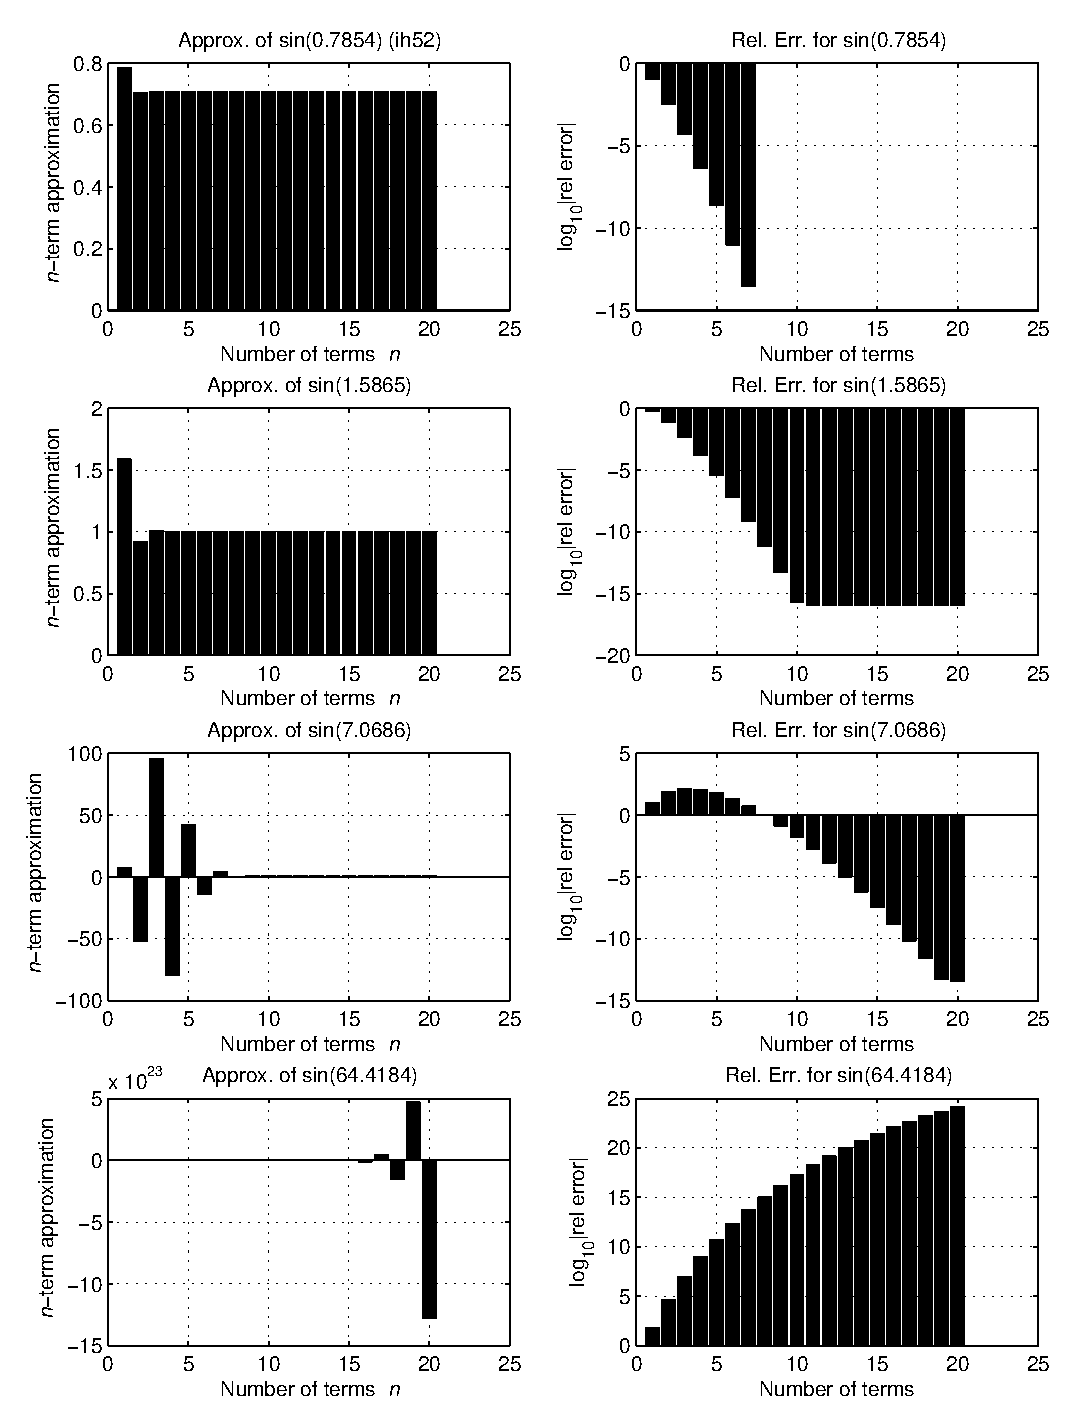
\epsfig{file=SinSeriesCheckerPlot.eps, width=6in}
\caption{Output of {\tt SinSeriesChecker.m} for Chapra 3.5}
\end{center}
\end{figure}

% As for the rest, 4.5in is usually fine
% Don't forget to remove % in front of \epsfig!
\begin{figure}[ht!]
\begin{center}
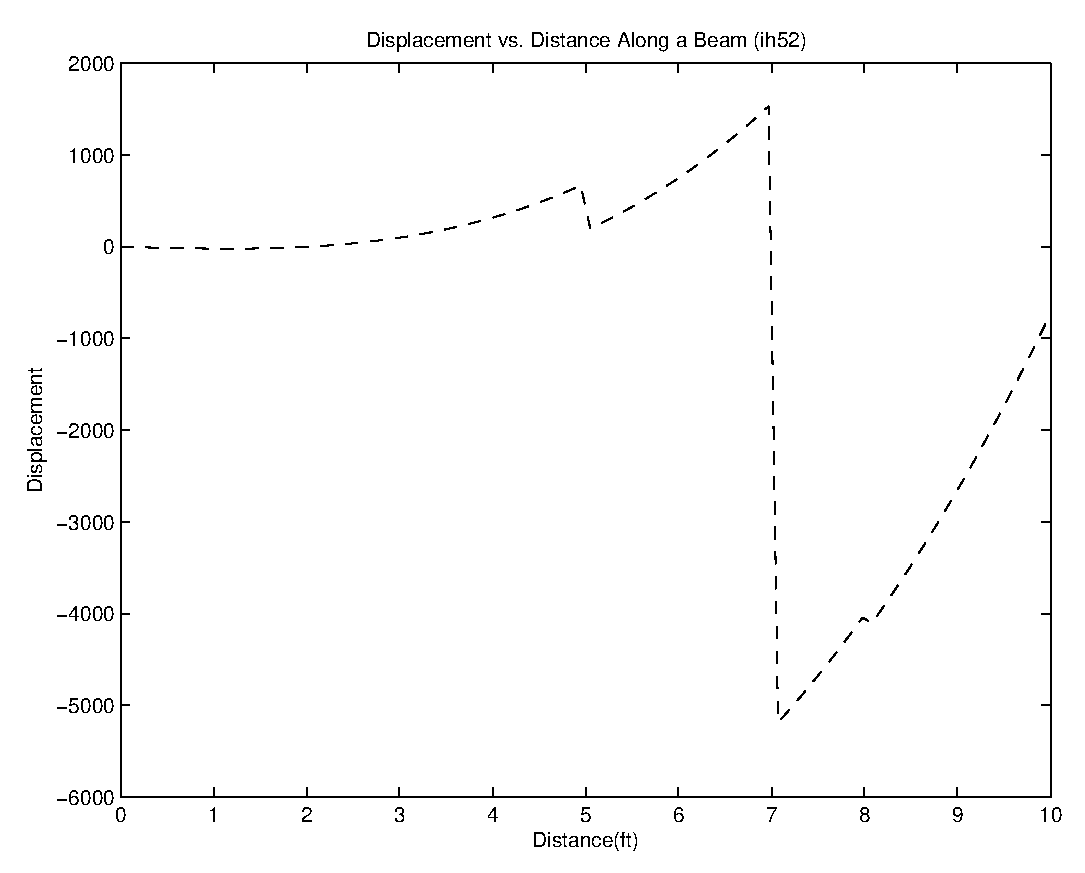
\epsfig{file=BeamDisplacement.eps, width=4.5in}
\caption{Beam Displacement versus Distance for Chapra 3.10}
\end{center}
\end{figure}

\begin{figure}[ht!]
\begin{center}
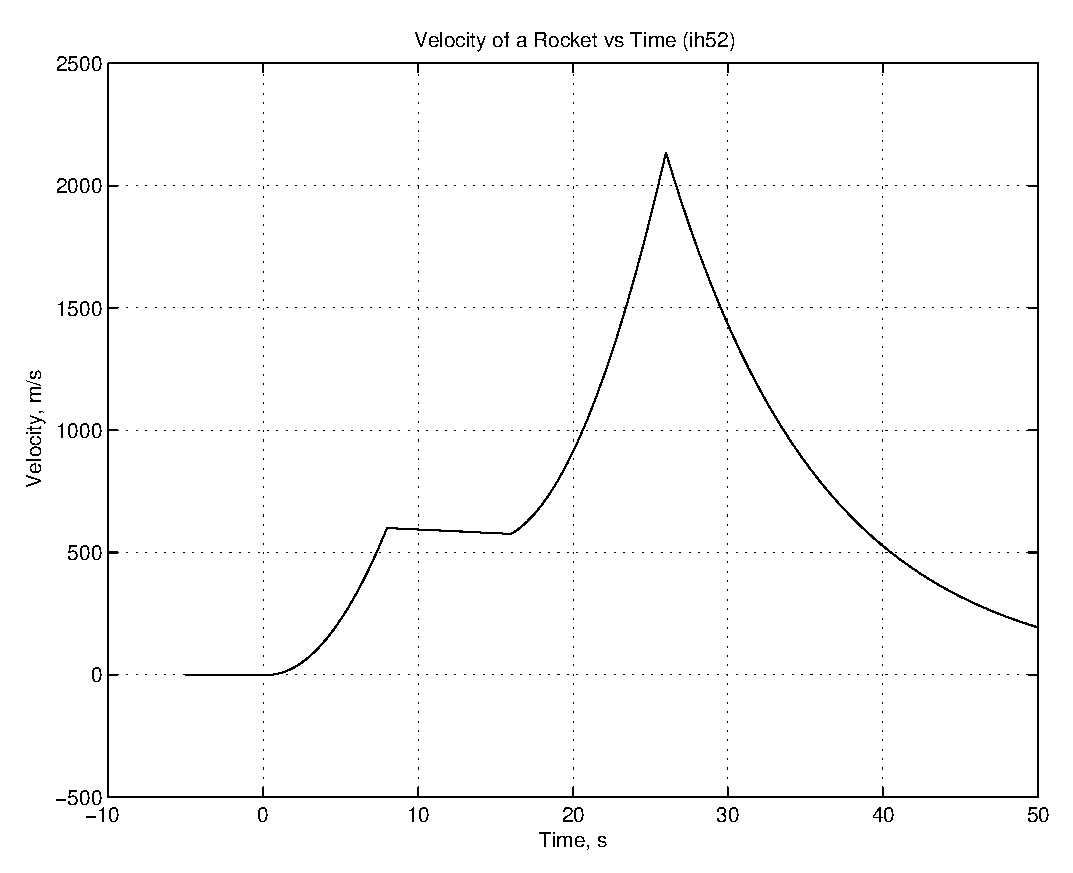
\epsfig{file=Chapra314.eps, width=4.5in}
\caption{Velocity of a Rocket vs. Time}
\end{center}
\end{figure}

\begin{figure}[ht!]
\begin{center}
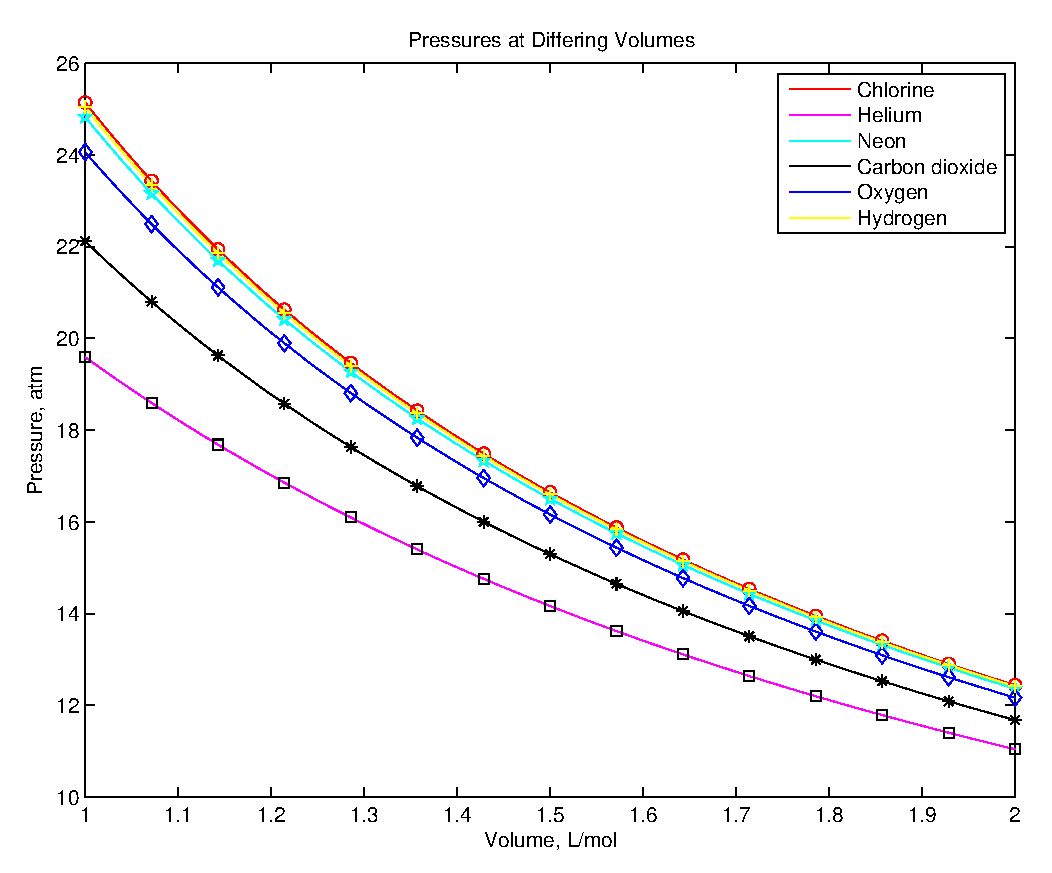
\epsfig{file=GraphPressures.eps, width=4.5in}
\caption{Pressures of Gases at Differing Volumes}
\end{center}
\end{figure}



\clearpage % start bibliography on new page

\begin{thebibliography}{9}
\bibitem{Chapra}
  Chapra, Steven C.,
  {\it Applied Numerical Methods with MATLAB for Engineering and Scientists}.
  McGraw-Hill, New York,
  3rd Edition,
  2012.
\bibitem{Palm}
  Palm, William J.,
  {\it Introduction to MATLAB for Engineers}.
  McGraw-Hill, New York,
  3rd Edition,
  2011.
\bibitem{Other}
  Weast, R.C. 
  {\it Van Der Waals Constants (Data Page)}
  Wikipedia, Wikimedia Foundation
  23 Sept. 2017

\end{thebibliography}

\end{document}
